\documentclass[12pt]{scrartcl}

 

\usepackage{float}

\usepackage[utf8]{inputenc}

\usepackage[T1]{fontenc}

\usepackage{lmodern}

\usepackage[ngerman]{babel}

\usepackage{amsmath}

\usepackage{graphicx}


 

\title{Versuch MI1\\ Mikrowellen}

\author{Frederik Strothmann, Henrik Jürgens}

\date{\today}


\begin{document}


 %deckblatt erstellen

\maketitle
\tableofcontents
\newpage

%einleitung zu dem experiment

\section{Einleitung}

Ein System aus Mikrowellensender und verschiedenen Empfängern ermöglicht Untersuchungen verschiedener physikalischer Effekte an Mikrowellen. So sollen in diesem Versuch stehende Wellen vermessen werden, außerdem wird die Wirkung einer Wachs-Sammellinse oder eines Polfilters (parallele Metallstäbe) untersucht sowie die Reflexion
an einer Wachsplatte (Brewster-Winkel), die Totalreflexion zwischen einer Wachs-Luft-
Wachs-Schicht und die Drehung der Polarisationsebene durch
”optisch aktive“ Substanzen.
(Spiralfedern in einem Styroporträger)
%versuchsaufbau mit skizze

\section{Versuchsaufbau}

%wenn du tabellen einfügst dann schreib bitte anstatt [htpb] [H]. zusammen mit \usepackage{float} verrutscht dann garnichts mehr
\section{Versuchsdurchführung}


\subsection{Praktische Durchführung}
\textbf{Allgemeine Hinweise:}\\
Die Mikrowellensender werden mit einer Gleichspannung von ca. 10 bis 12 V versorgt.
Polung beachten und niemals höhere Spannungen anlegen! Niemals darf an die Mikrowellenempfänger versehentlich eine Gleichspannung angelegt werden! Das würde die empfindliche Diode sofort zerstören.
\begin{enumerate}
\item Stellen Sie den Sender und eine Metallplatte im Abstand von ca. 30 - 40 cm gegenüber auf und zwischen beide die Diode. Stellen Sie so eine stehende Welle her
und messen Sie durch Verschieben der Metallplatte die Wellenlänge.
\item
Überzeugen Sie sich von den Eigenschaften einer Sammellinse, indem Sie die Intensitätsverteilung senkrecht zur Strahlrichtung mit dem Hornempfänger messen:
\begin{enumerate}
\item ohne Linse (Abstand Sender-Empfänger ca. 1,5 m)
\item mit Linse (Abstand Sender-Linse 0,5 m, Linse-Empfänger 1 m)
\end{enumerate}
\item Zeigen Sie die Totalreflexion anhand des folgenden Versuchs:

%hier die Abbildung aus der Versuchsanleitung einfügen, footnote muss noch geschrieben werden.
\begin{figure}[htbp] 
  \centering
    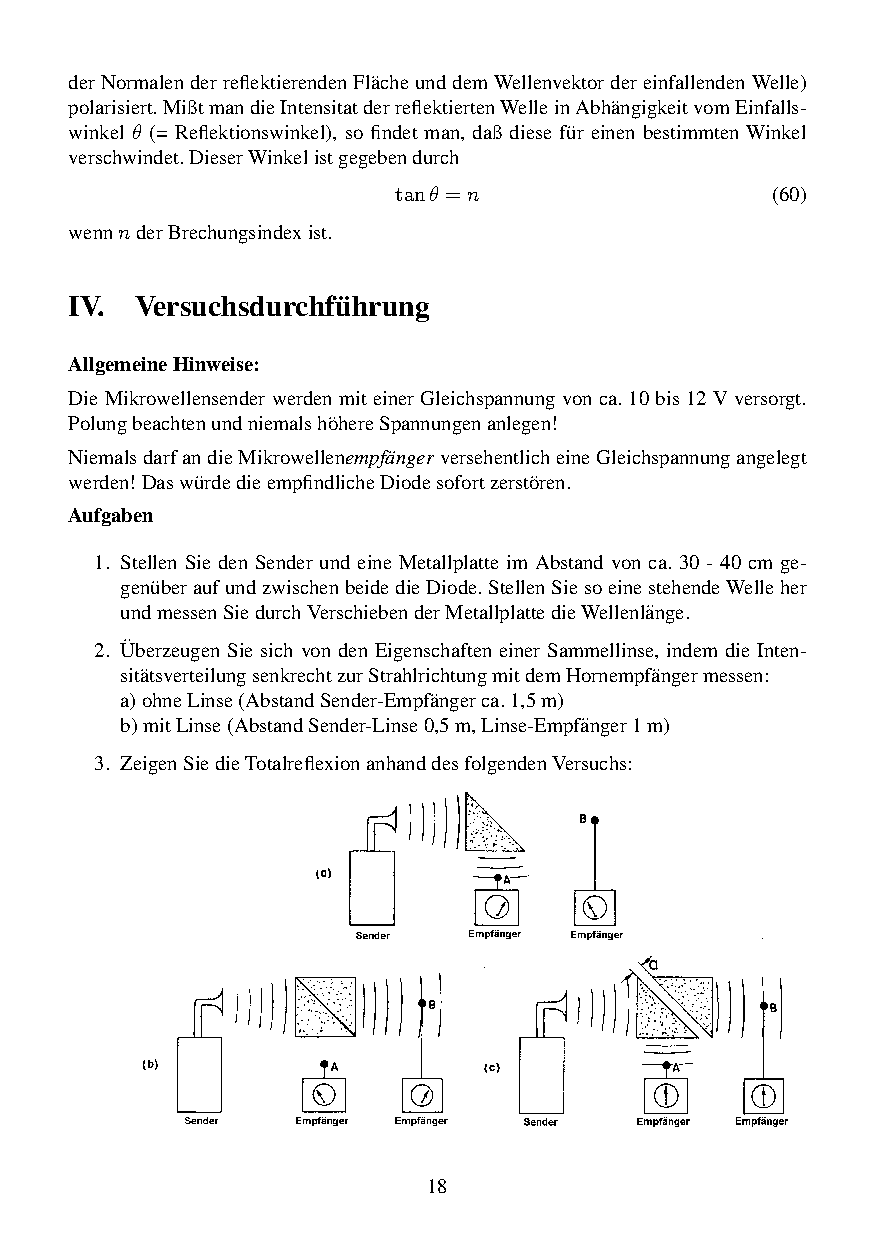
\includegraphics[trim = 80mm 15mm 0mm 160mm, clip, scale = 1]{totalreflexion.pdf}
  	\caption[Abbildung der beiden Schaltungen, für die Bestimmung des Wiederstandes]{Abbildung der beiden Schaltungen, für die Bestimmung des Wiederstandes\footnotemark}
  \label{fig:abb_versuch_3}
\end{figure}
\footnotetext{Abbildung entnommen von http://www.atlas.uni-wuppertal.de/~kind/MI1.pdf Seite 18 am 16.08.2014}

Stellen Sie die Wachsprismen ( n = 1,5 ) wie in der Abbildung (c) gezeichnet im Abstand a gegenüber. Messen Sie die Intensität des Empfängers in Abhängigkeit von Abstand a. Versuchen Sie, die Erscheinung zu erklären.
\item Stellen Sie Sender und Empfänger gegenüber, so dass die Polarisationsrichtungen
(Richtungen, in denen der E-Vektor schwingt) der beiden parallel sind. Drehen Sie dann den Empfänger um die Verbindungslinie von Sender und Empfänger und messen Sie dabei die Intensität in Abhängigkeit des Drehwinkels.
\item Stellen Sie Sender und Empfänger um 90$^{\circ}$ gedreht gegenüber. Halten Sie dann ein Gitter zwischen Sender und Empfänger, so dass die Stäbe mit dem E-Vektor einen Winkel von 45$^{\circ}$ bilden.
\item Messen Sie die Intensität der von einer Wachsplatte reflektierten Wellen, die parallel zur Einfallsebene polarisiert sind, in Abhängigkeit vom Einfallswinkel. Bestimmen Sie den Brechungsindex.
\item Zeigen Sie die Drehung der Polarisationsebene durch ”optisch aktive“ Substanzen. Es gibt dazu zwei Sorten optisch aktiver Substanz, nämlich Federn in Styroporplatten, mit Links- bzw. Rechtsschraube. Die Platten sind durch eine Markierung (L und R) an der Seite der Styroporplatten einfach zu unterscheiden.
\end{enumerate}

\subsection{Theoretische Durchführung}


\section{Messergebnisse}



\section{Auswertung}


\section{Diskussion}


 %Werte stimmen mit den Formeln überein/nicht überein

\end{document}

